\documentclass[12pt]{article}


\usepackage{amssymb}
\usepackage{amsmath}
\usepackage{fullpage}
\usepackage{epsfig}
\usepackage{epstopdf, hyperref, xcolor}
\everymath{\displaystyle}
\usepackage{enumerate}

\newif\ifans

\anstrue

\begin{document}

\begin{center}
\underline{\LARGE{Polar Coordinates}}
\end{center}

\noindent SUGGESTED REFERENCE MATERIAL:

\bigskip

\noindent As you work through the problems listed below, you should reference Chapter 10.2 of the recommended textbook (or the equivalent chapter in your alternative textbook/online resource) and your lecture notes.

\bigskip

\noindent EXPECTED SKILLS:

\begin{itemize}

\item Be able to describe points and curves in both polar and rectangular form, and be able to convert between the two coordinate systems. 

\item Know the formulas for the basic shapes in polar coordinates: circles, lines, limacons, cardioids, rose curves,
and spirals.

\end{itemize}

\noindent PRACTICE PROBLEMS:

\medskip

\noindent {\bf For problems 1-6, compute the rectangular coordinates of the points whose polar coordinates are given.} 

\begin{enumerate}

\item $\left(-1, \frac{\pi}{3}\right)$ 

\ifans{\fbox{$\left(-\frac{1}{2},-\frac{\sqrt{3}}{2}\right)$}} \fi

\item $\left(3, \frac{2\pi}{3}\right)$ 

\ifans{\fbox{$\left(-\frac{3}{2},\frac{3\sqrt{3}}{2}\right)$}} \fi

\item $(5, -\pi)$ 

\ifans{\fbox{$(-5,0)$}} \fi

\item $\left(-2, \frac{9\pi}{4}\right)$ 

\ifans{\fbox{$\left(-\sqrt{2},-\sqrt{2}\right)$}} \fi

\item $\left(6, \frac{11\pi}{6}\right)$ 

\ifans{\fbox{$\left(3\sqrt{3},-3\right)$}} \fi

\end{enumerate}

\newpage

\noindent {\bf For problems 7-11, find two pairs of polar coordinates for the point whose rectangular coordinates are given.  The first pair should satisfy $r \geq 0$ and $0 \leq \theta <2\pi$.  The second pair should satisfy $r \geq 0$ and $-2\pi<\theta \leq 0$.}

\begin{enumerate}
\setcounter{enumi}{6}

\item $(-5, -5)$ 

\ifans{\fbox{I. $\left(5\sqrt{2},\frac{5\pi}{4}\right)$; II. $\left(5\sqrt{2},-\frac{3\pi}{4}\right)$}} \fi

\item $(-3, 3)$ 

\ifans{\fbox{I. $\left(3\sqrt{2},\frac{3\pi}{4}\right)$; II. $\left(3\sqrt{2},-\frac{5\pi}{4}\right)$}} \fi

\item $(0,3)$ 

\ifans{\fbox{I. $\left(3,\frac{\pi}{2}\right)$; II. $\left(3,-\frac{3\pi}{2}\right)$}} \fi

\item $\left(\sqrt{3}, -1\right)$ 

\ifans{\fbox{I. $\left(2,\frac{11\pi}{6}\right)$; II. $\left(2,-\frac{\pi}{6}\right)$; Detailed Solution: \textcolor{blue}{\href{http://www.math.drexel.edu/classes/Calculus/resources/Math122HW/Solutions/122_18_Polar_10.pdf}{Here}}}} \fi

\item $\left(-4\sqrt{3}, -4\right)$ 

\ifans{\fbox{I. $\left(8,\frac{7\pi}{6}\right)$; II. $\left(8,-\frac{5\pi}{6}\right)$}} \fi

\item Consider the point with rectangular coordinates $\left(1,\sqrt{3}\right)$.

\begin{enumerate}

\item Find a pair of polar coordinates which satisfy $r \geq 0$ and $0 \leq \theta< 2\pi$

\ifans{\fbox{$(r,\theta)=\left(2,\frac{\pi}{3}\right)$}} \fi

\item Find a pair of polar coordinates which satisfy $r \leq 0$ and $0 \leq \theta <2\pi$

\ifans{\fbox{$(r,\theta)=\left(-2,\frac{4\pi}{3}\right)$}} \fi

\item Find a pair of polar coordinates which satisfy $r \geq 0$ and $-2\pi < \theta \leq 0$

\ifans{\fbox{$(r,\theta)=\left(2,-\frac{5\pi}{3}\right)$; }} \fi

\item Find a pair of polar coordinates which satisfy $r \leq 0$ and $-2\pi < \theta \leq 0$

\ifans{\fbox{$(r,\theta)=\left(-2,-\frac{2\pi}{3}\right)$}} \fi

\end{enumerate}

\end{enumerate}

\noindent {\bf For problems 13-17, identify the curve by transforming the polar equation into rectangular coordinates.} 

\begin{enumerate}
\setcounter{enumi}{12}

\item $r=1$ 

\ifans{\fbox{circle, $x^2+y^2=1$}} \fi

\item $r=2\cos{\theta}$ 

\ifans{\fbox{circle, $(x-1)^2+y^2=1$}} \fi

\item $r\sin{\theta}=2$ 

\ifans{\fbox{line, $y=2$}} \fi

\item $r=3\cos{\theta}-2\sin{\theta}$

\ifans{\fbox{circle, $\left(x-\frac{3}{2}\right)^2+(y+1)^2=\frac{13}{4}$; Detailed Solution: \textcolor{blue}{\href{http://www.math.drexel.edu/classes/Calculus/resources/Math122HW/Solutions/122_18_Polar_16.pdf}{Here}}}}\fi

\item $r=6\sec{\theta}$

\ifans{\fbox{line, $x=6$}} \fi

\end{enumerate}

\noindent{\bf For problems 18-21, express the given equation in polar coordinates.}

\begin{enumerate}
\setcounter{enumi}{17}
\item $y=2$ 

\ifans{\fbox{$r=2\csc{\theta}$}} \fi

\item $x=3$ 

\ifans{\fbox{$r=3\sec{\theta}$; Detailed Solution: \textcolor{blue}{\href{http://www.math.drexel.edu/classes/Calculus/resources/Math122HW/Solutions/122_18_Polar_19.pdf}{Here}}}} \fi

\item $x^2+y^2=10$ 

\ifans{\fbox{$r=\sqrt{10}$}} \fi

\item $x^2+y^2+8y=0$

\ifans{\fbox{$r=-8\sin{\theta}$}} \fi

\end{enumerate}

\newpage

\noindent {\bf For problems 22-24, find an equation in polar coordinates for each of the given graphs.}

\begin{enumerate}
\setcounter{enumi}{21}

\item Circle:\\
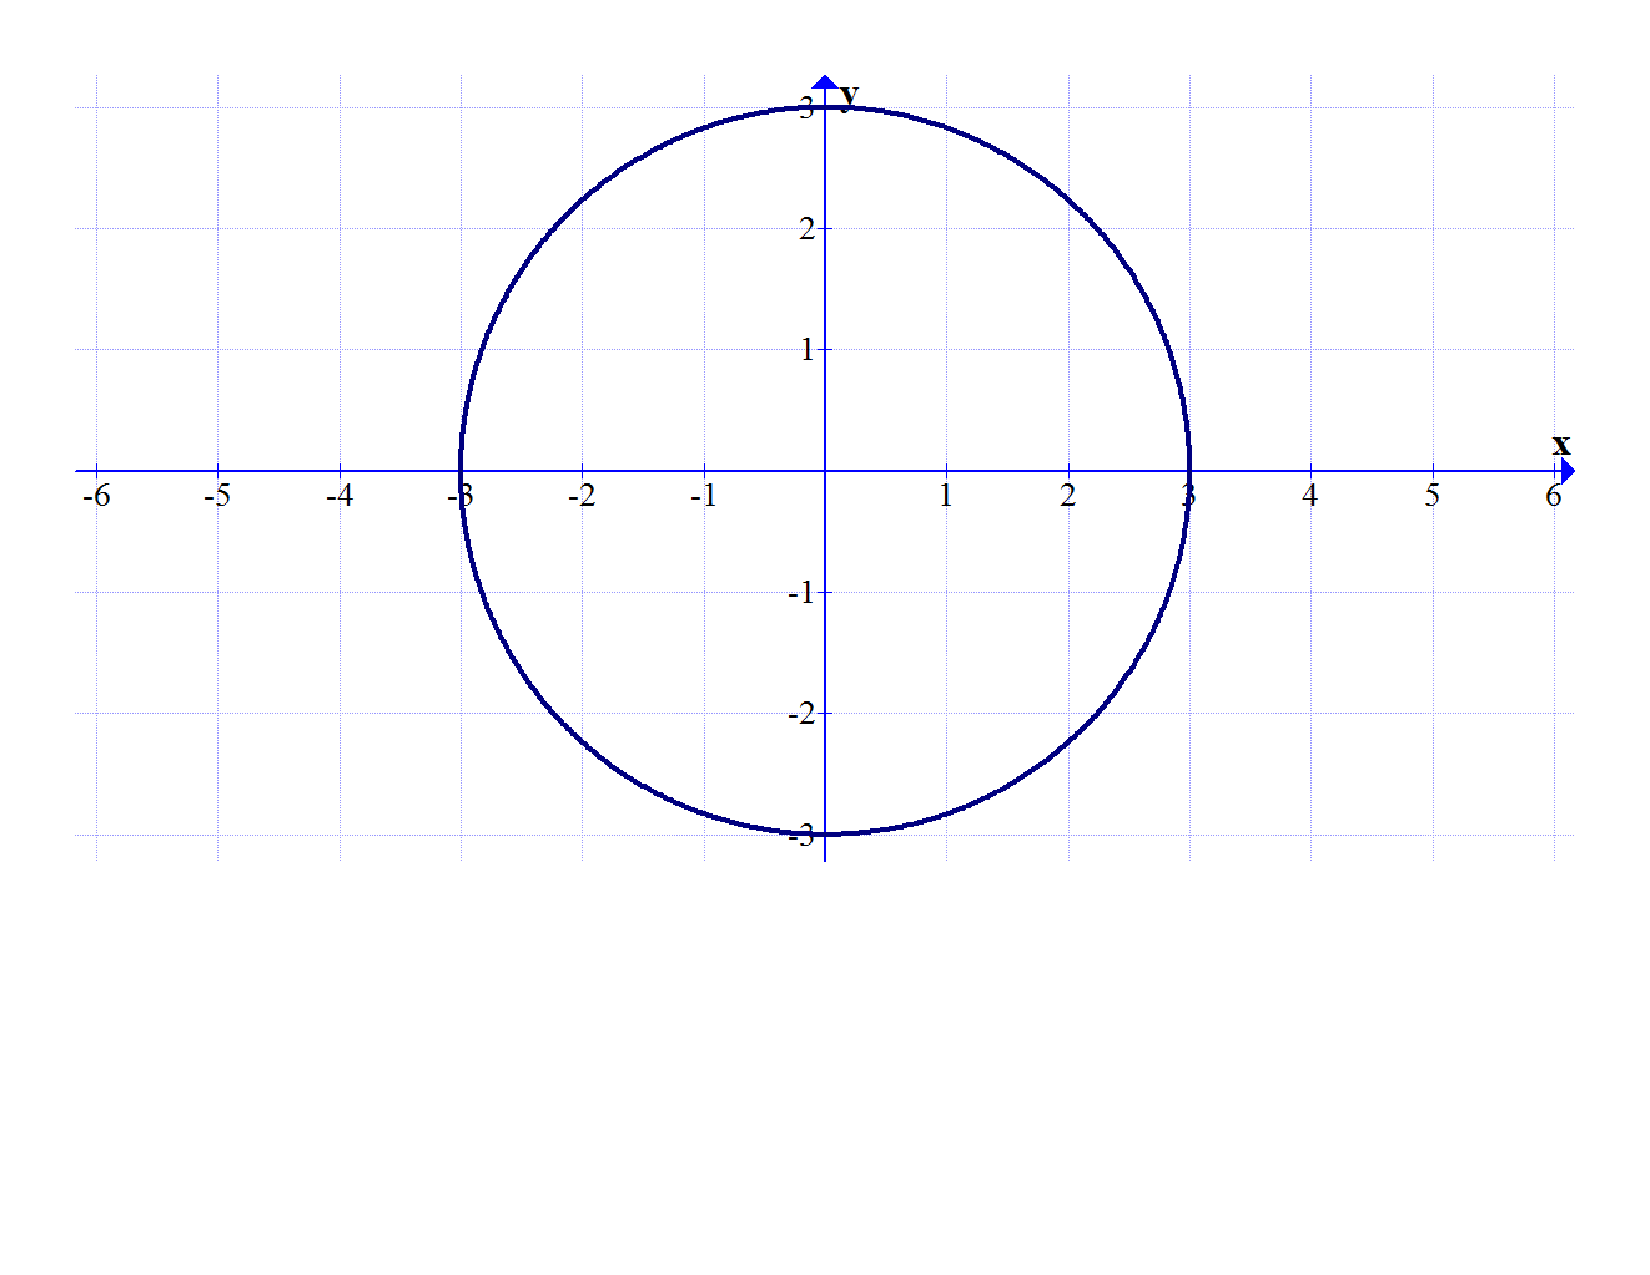
\includegraphics[scale=0.35]{graph1.pdf}

\ifans{\fbox{$r=3$}} \fi

\item Circle\\
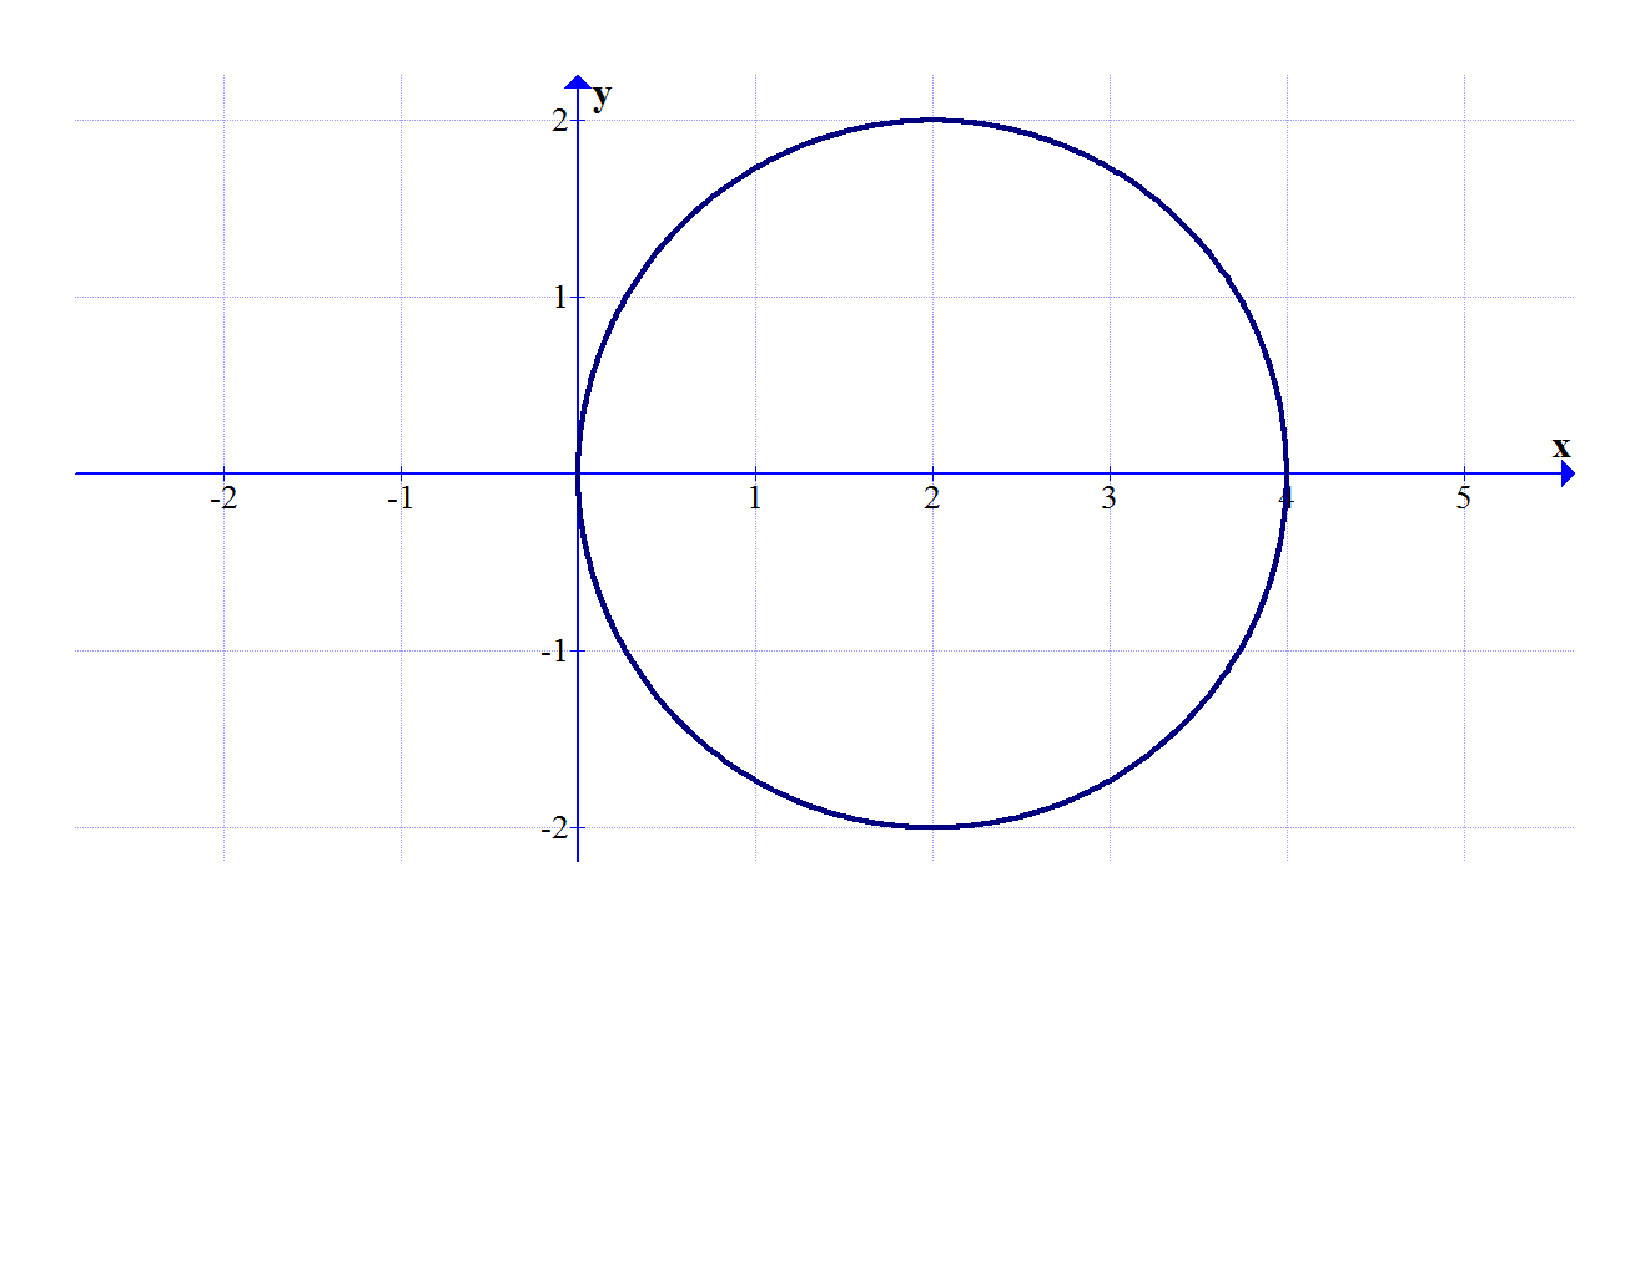
\includegraphics[scale=0.35]{graph2.pdf}

\ifans{\fbox{$r=4\cos{\theta}$}} \fi

\item Cardioid\\
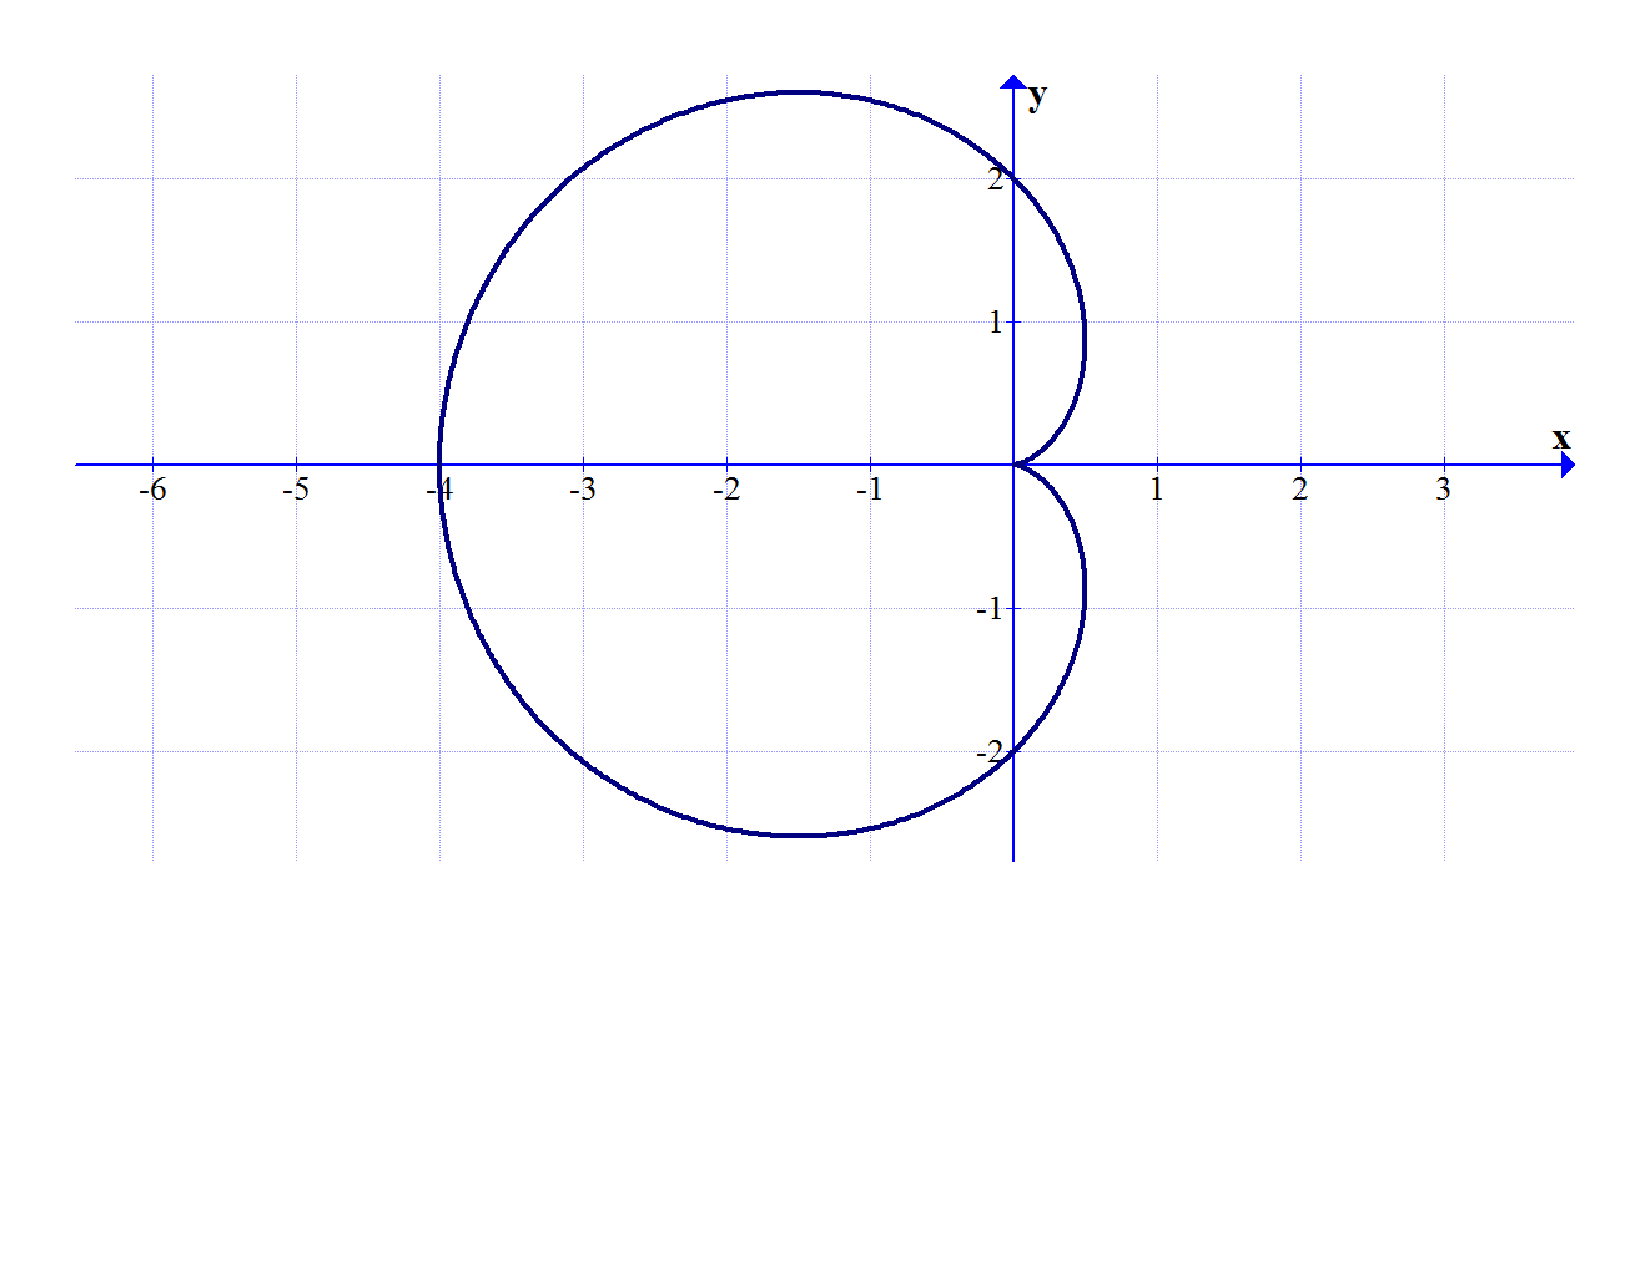
\includegraphics[scale=0.35]{graph3.pdf}

\ifans{\fbox{$r=2(1-\cos{\theta})$}} \fi

\end{enumerate}

\newpage

\noindent{\bf For problems 25-34, sketch the curve in polar coordinates.}

\begin{enumerate}
\setcounter{enumi}{24}

\item $r=2$ 

\ifans{\fbox{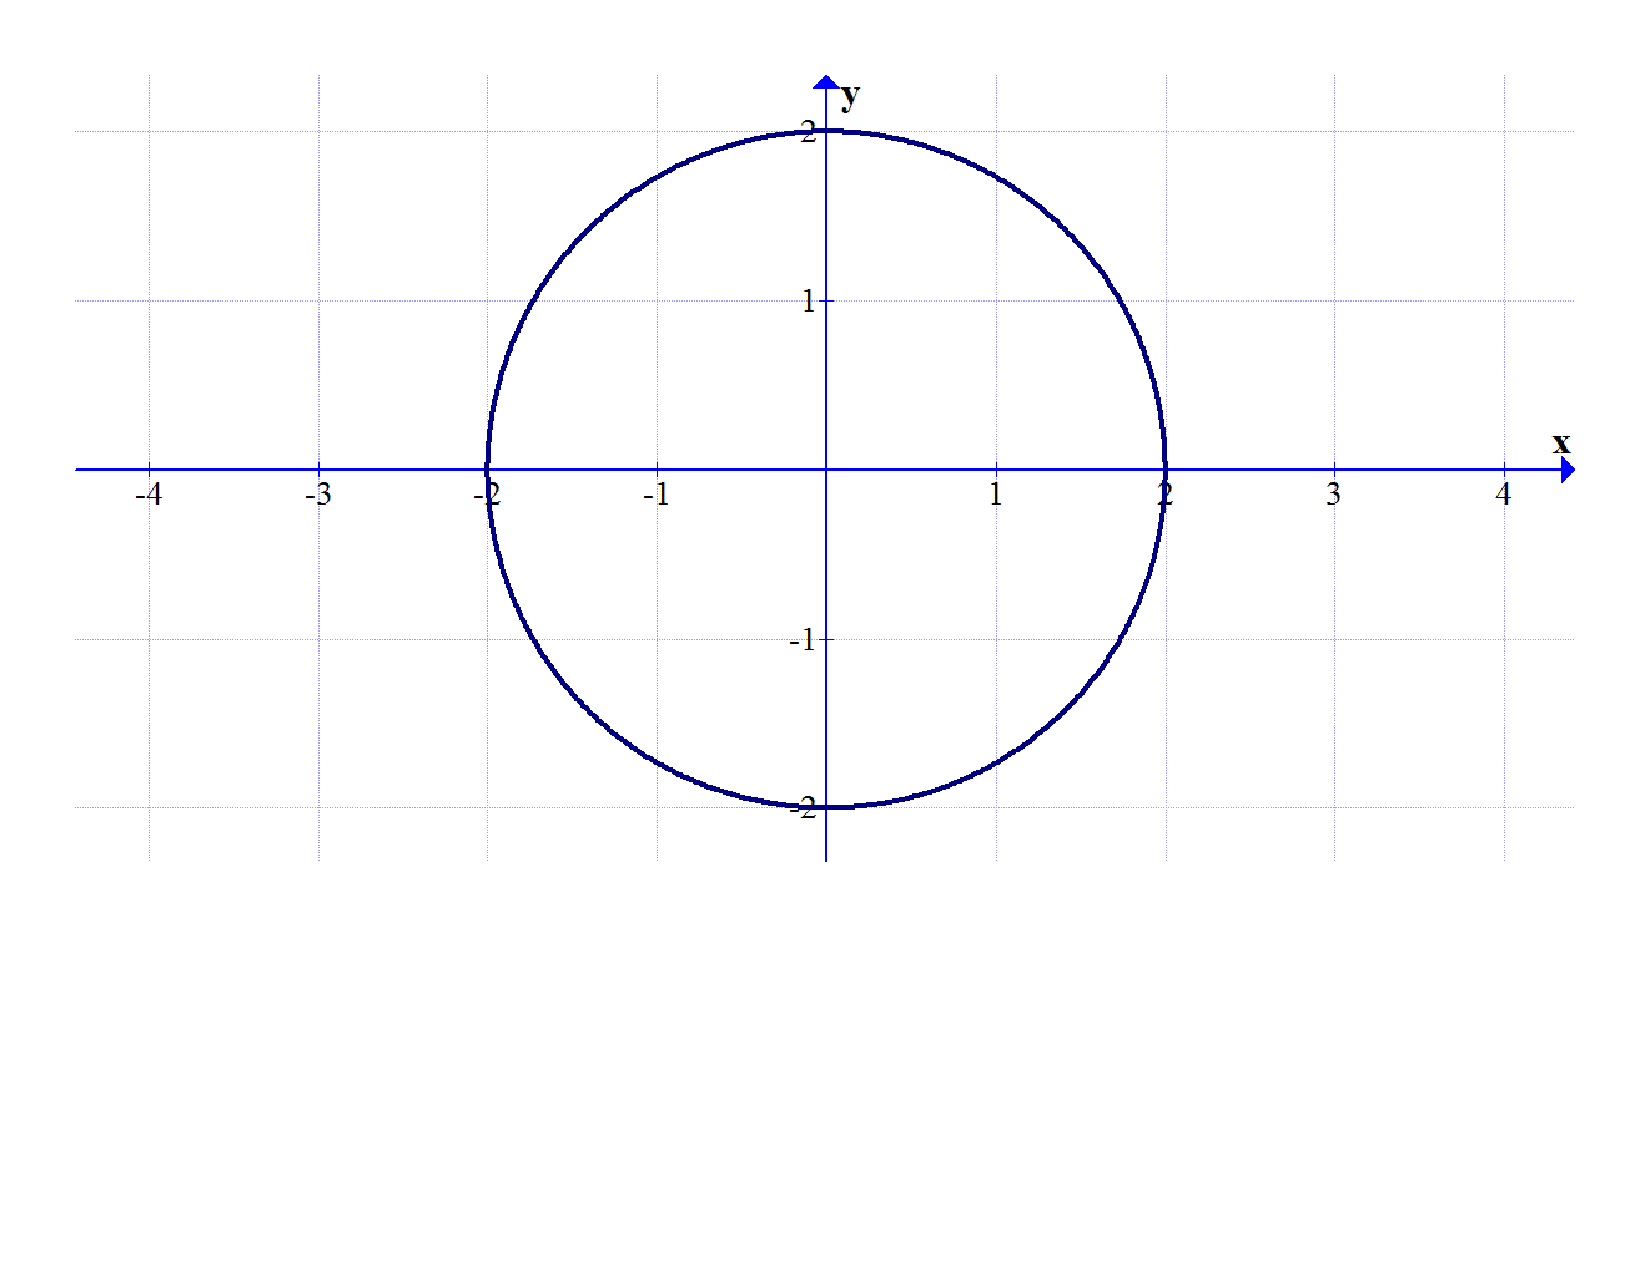
\includegraphics[scale=0.27]{sketch1}}} \fi

\item $r=\cos{\theta}$ 

\ifans{\fbox{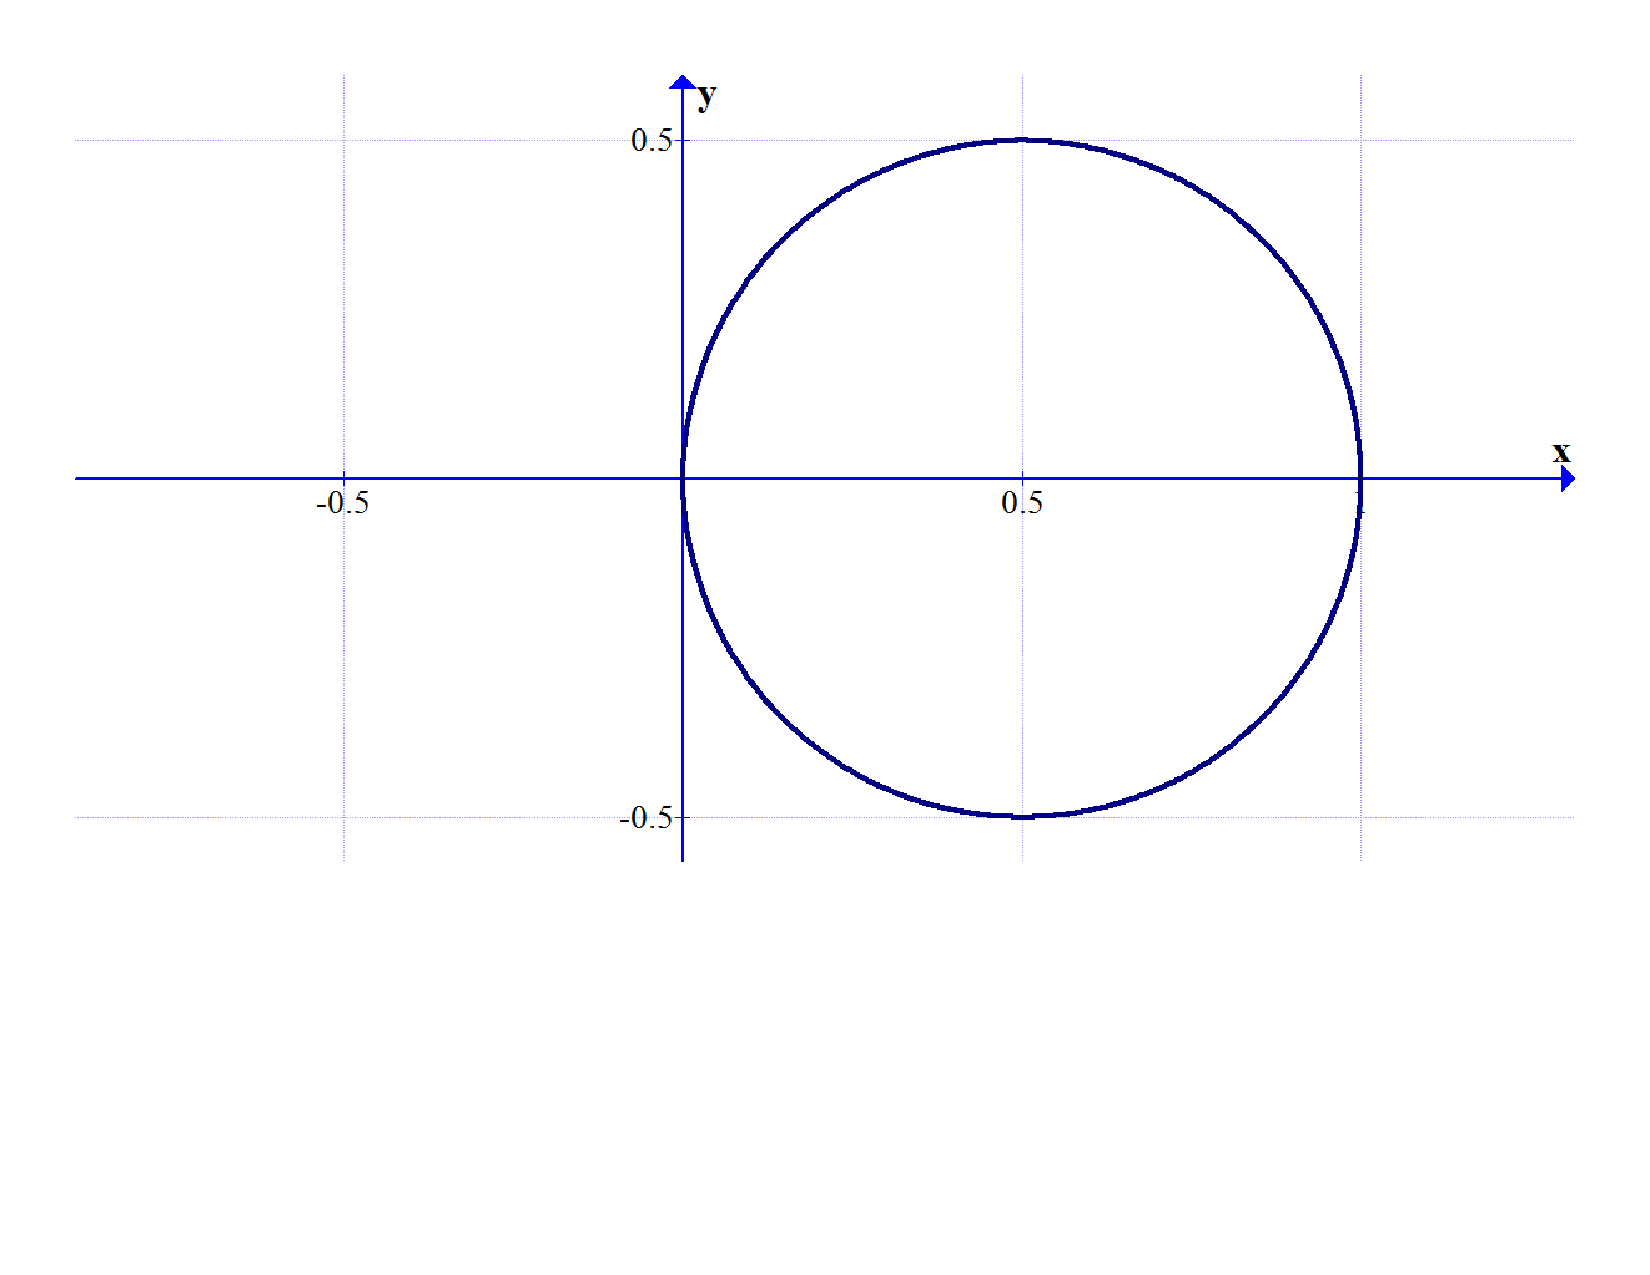
\includegraphics[scale=0.27]{sketch2.pdf}}} \fi

\item $r=3\sin{\theta}$ 

\ifans{\fbox{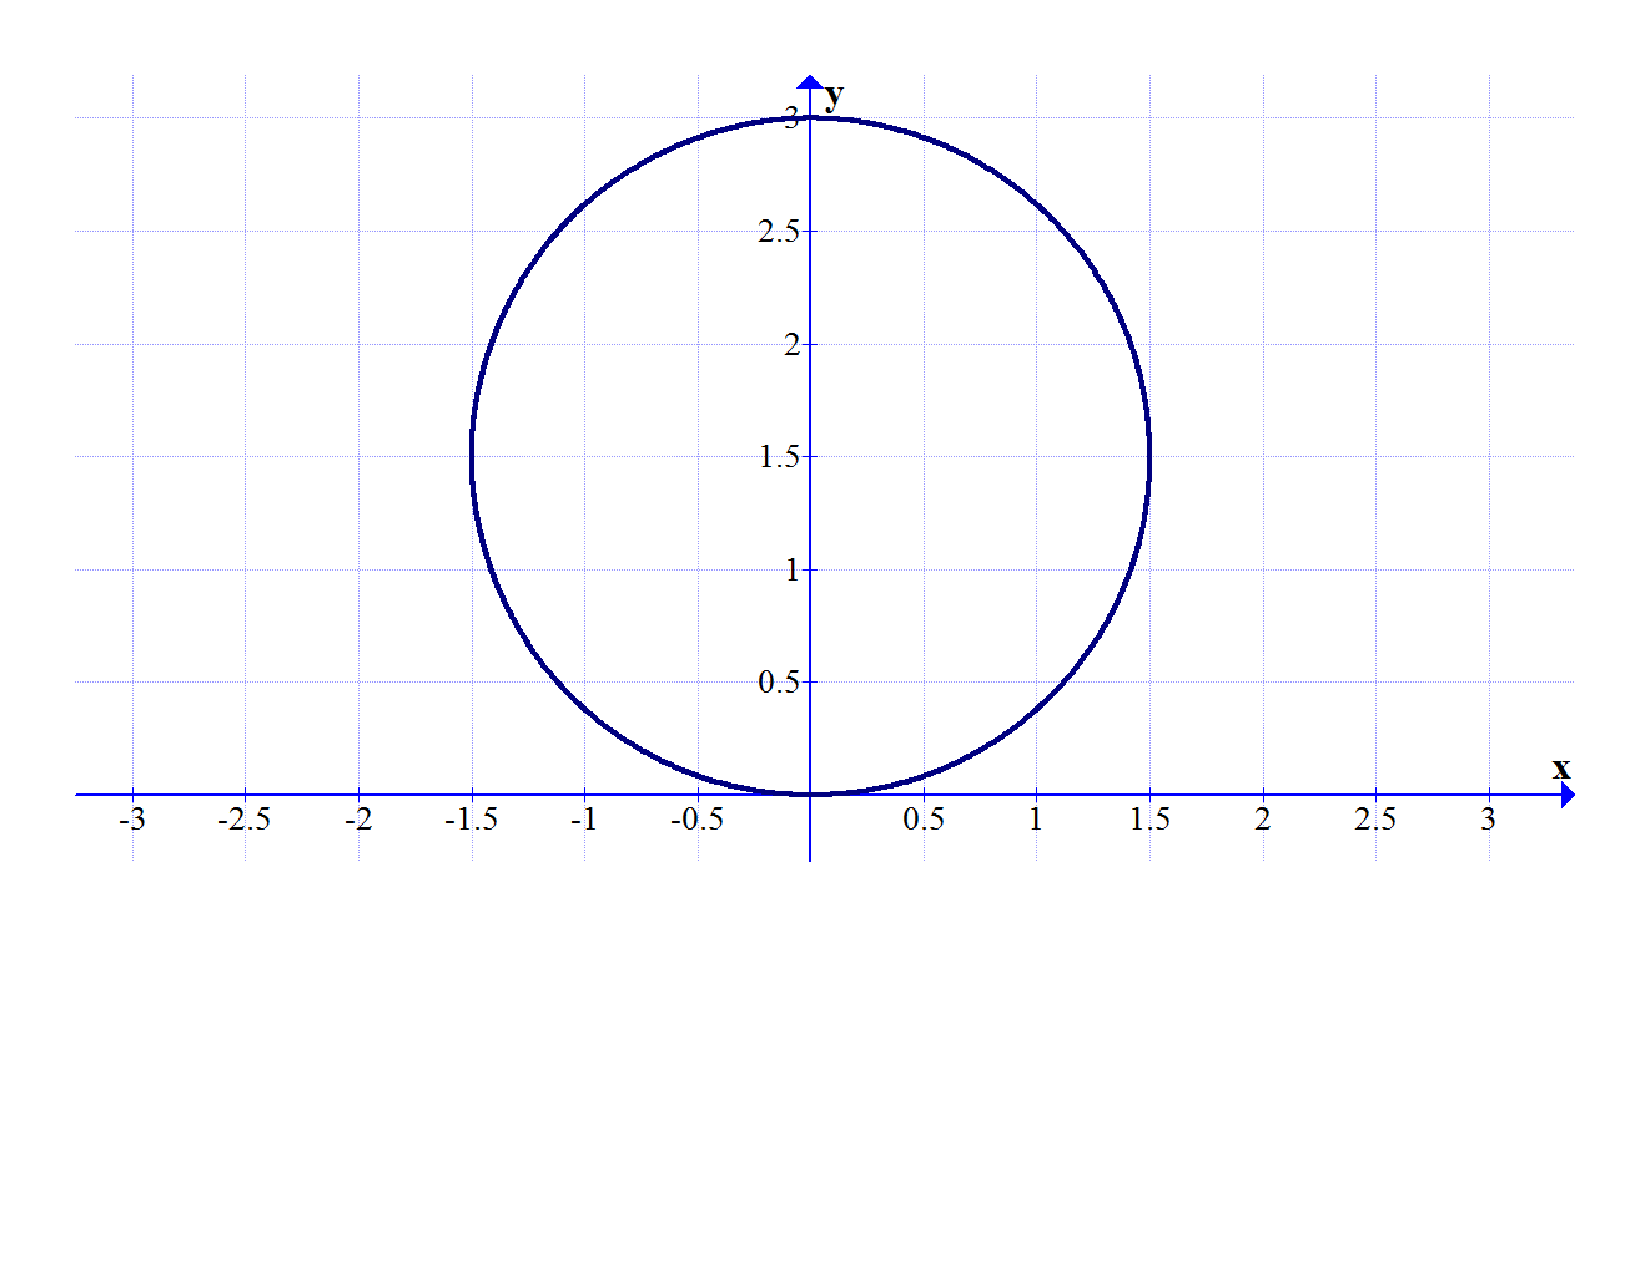
\includegraphics[scale=0.27]{sketch3.pdf}}} \fi

\item $r=3+3\sin{\theta}$ 

\ifans{\fbox{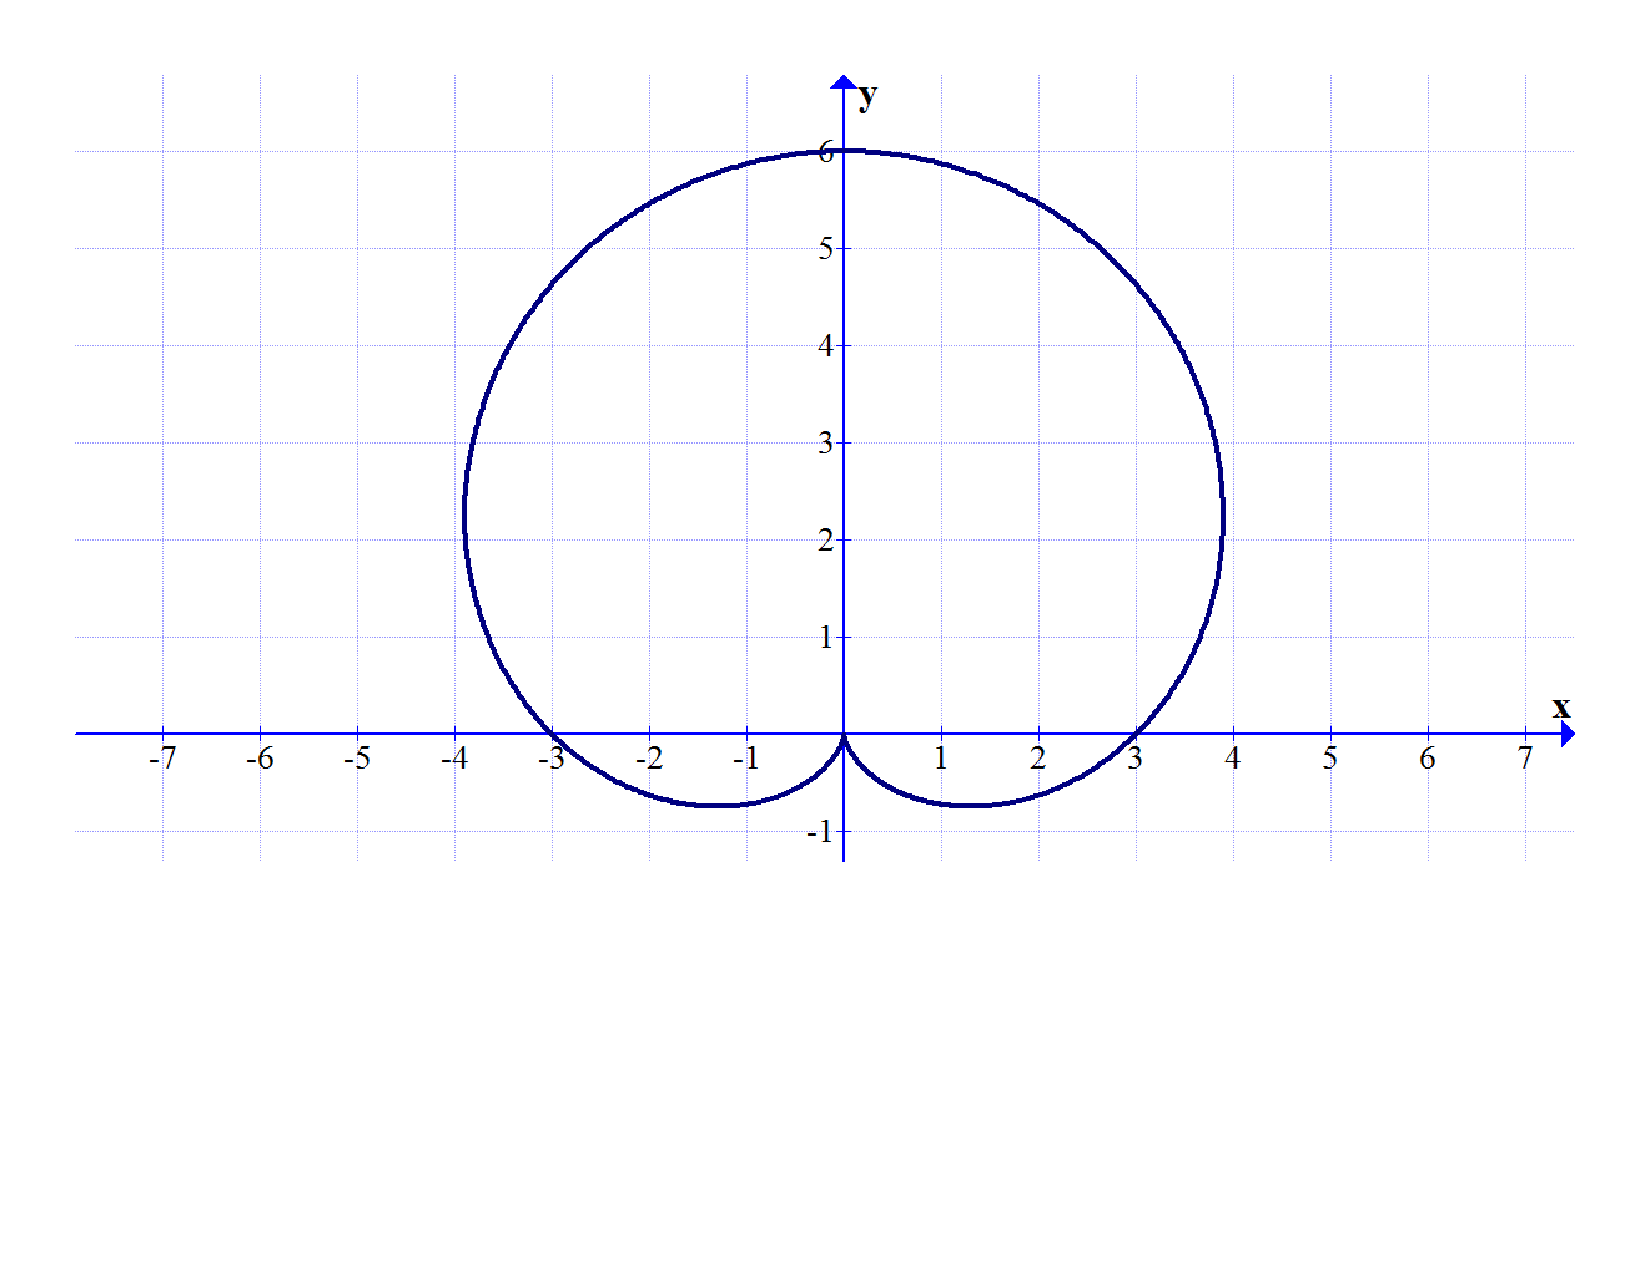
\includegraphics[scale=0.27]{sketch4.pdf}}} \fi

\newpage

\item $r=1-2\cos{\theta}$ 

\ifans{\fbox{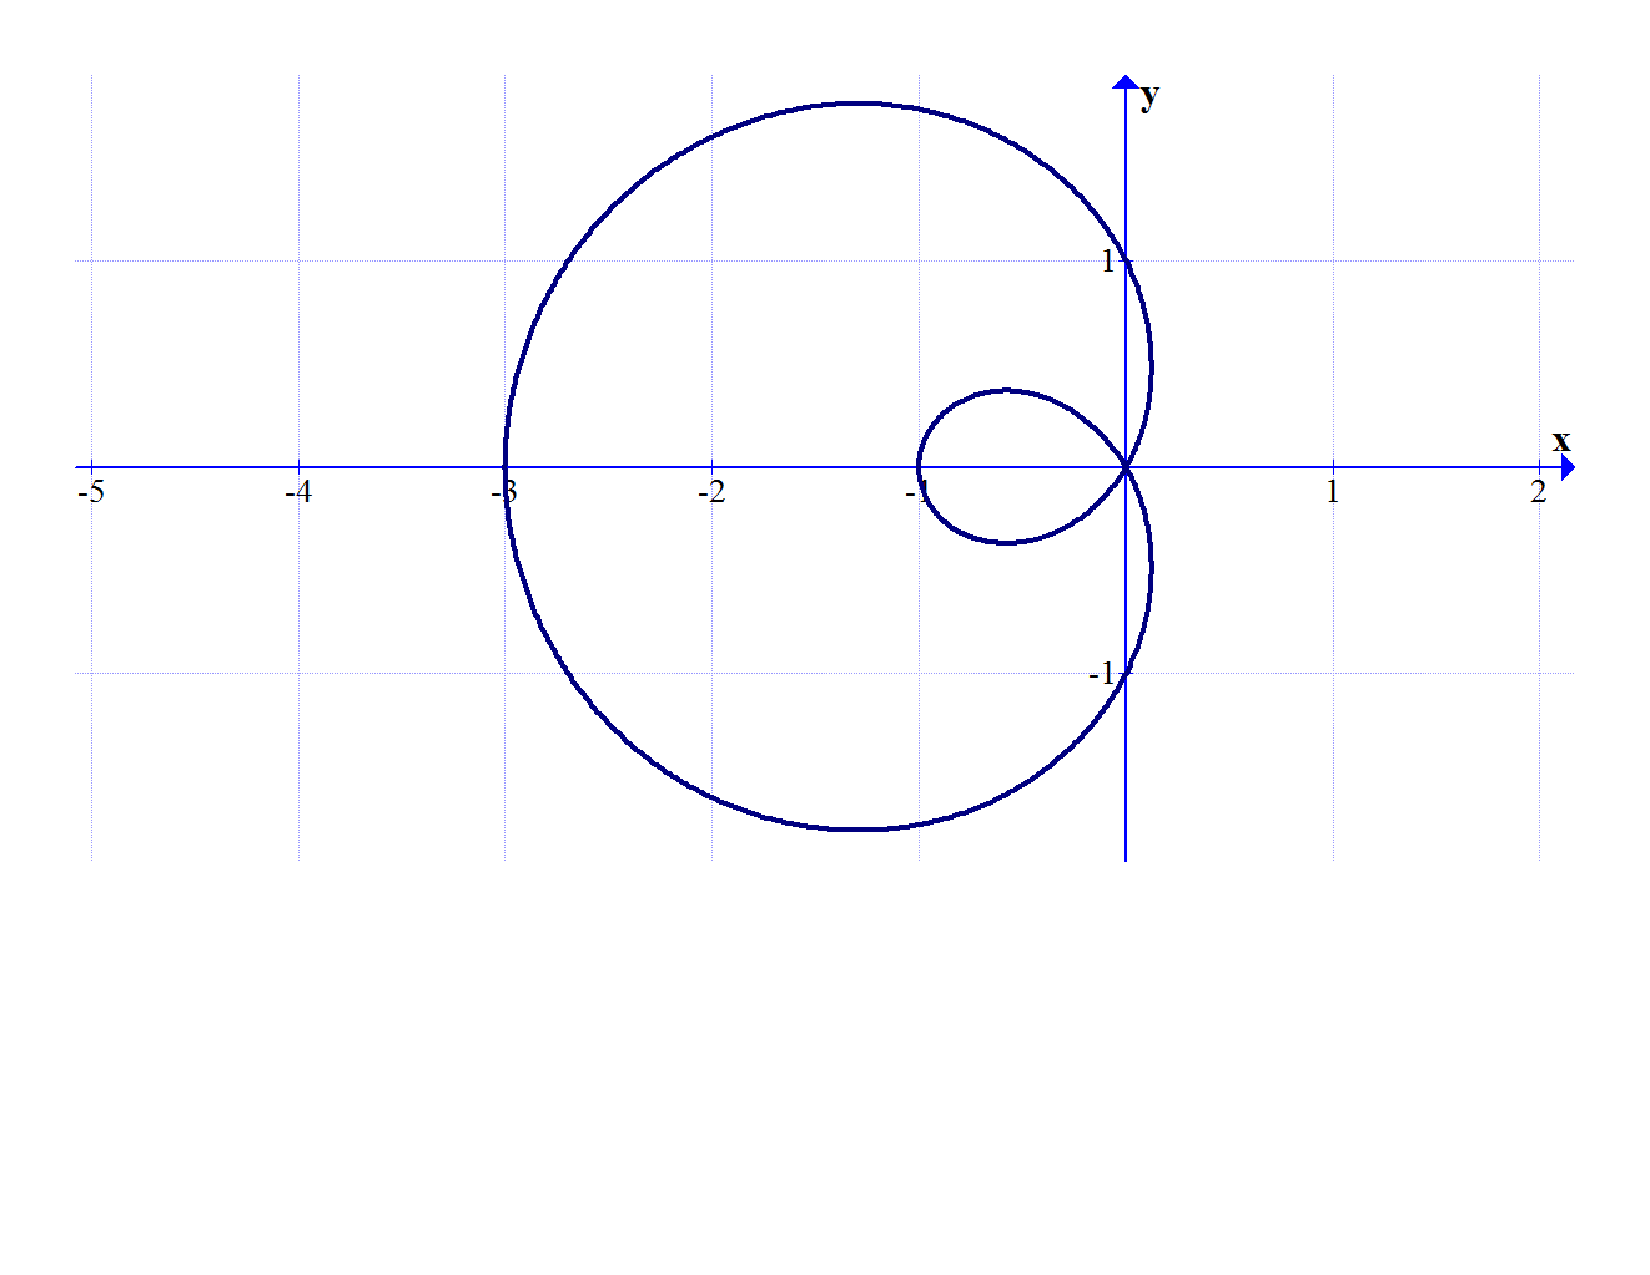
\includegraphics[scale=0.27]{sketch5.pdf}}} \fi

\item $r=3\theta$, $0 \leq \theta \leq 2\pi$

\ifans{\fbox{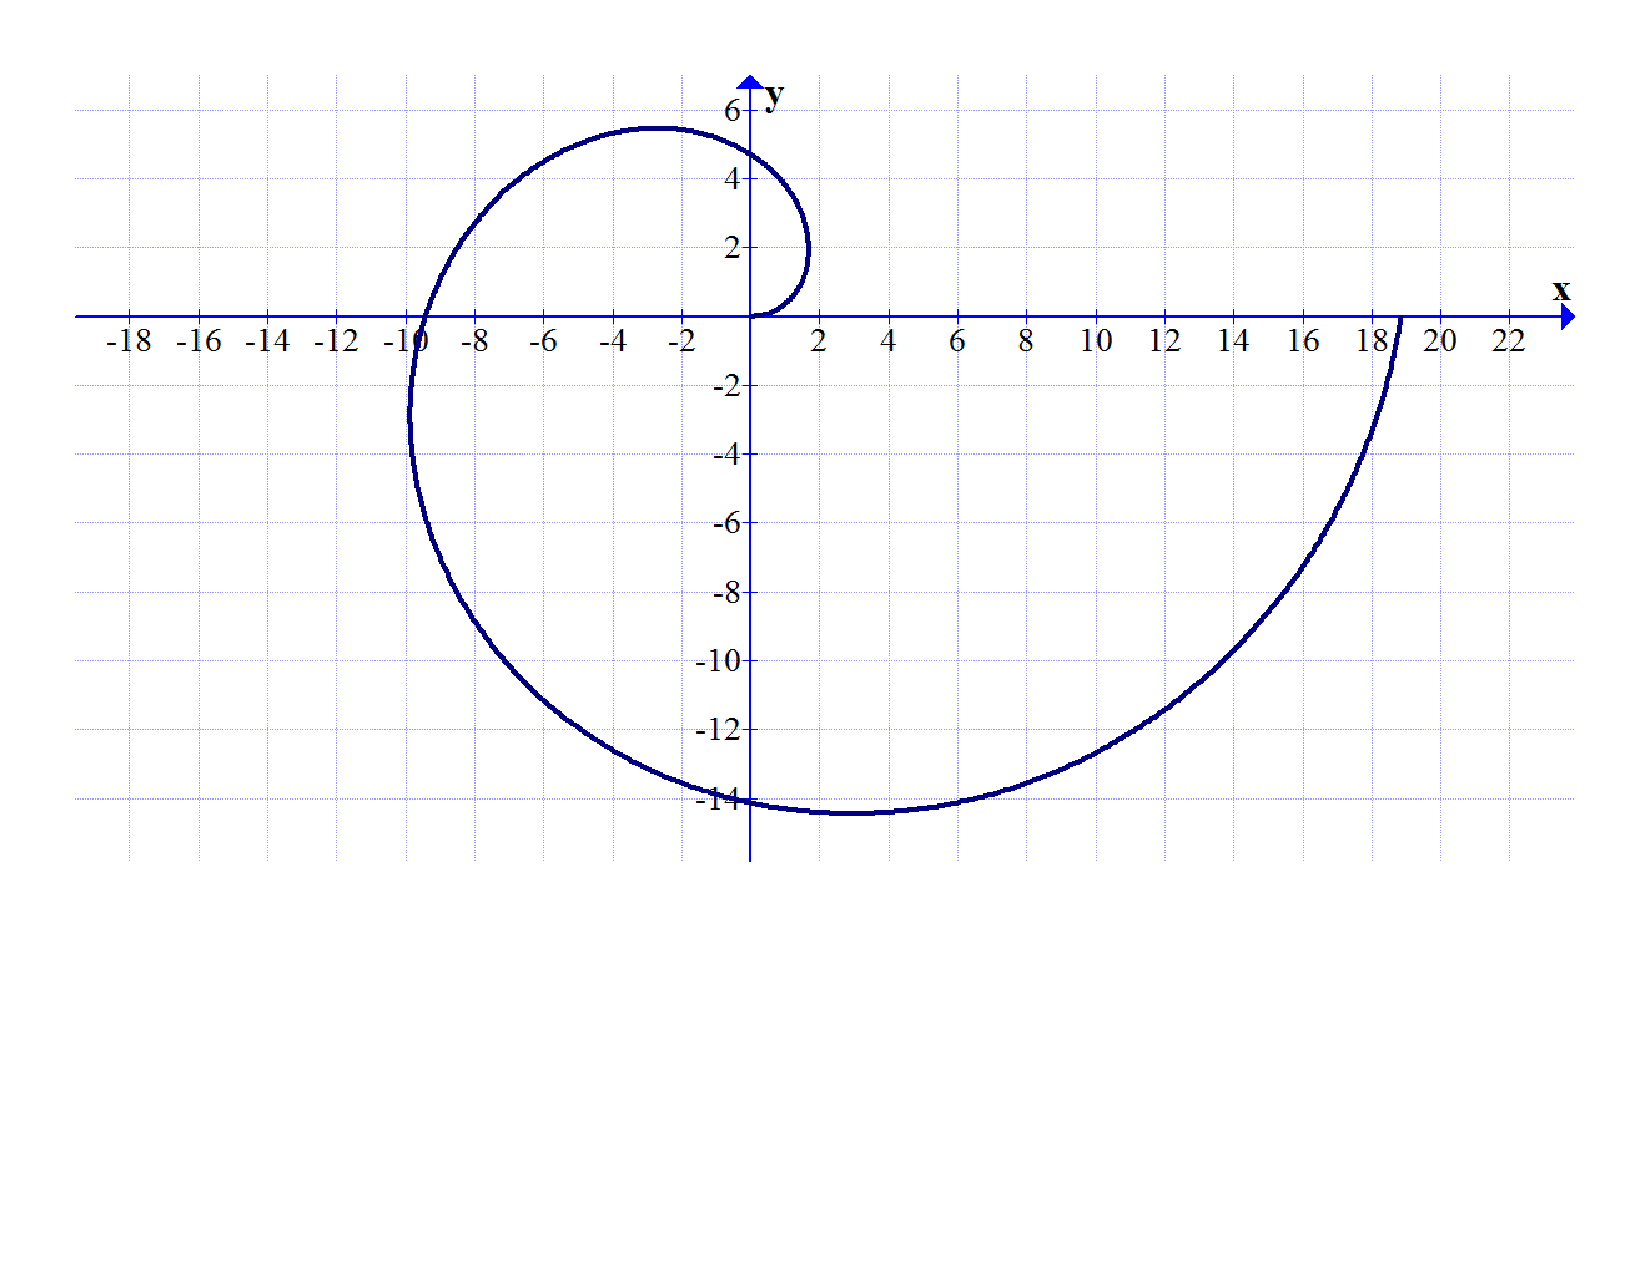
\includegraphics[scale=0.27]{sketch6.pdf}}} \fi

\item $r=2-3\sin{\theta}$ 

\ifans{\fbox{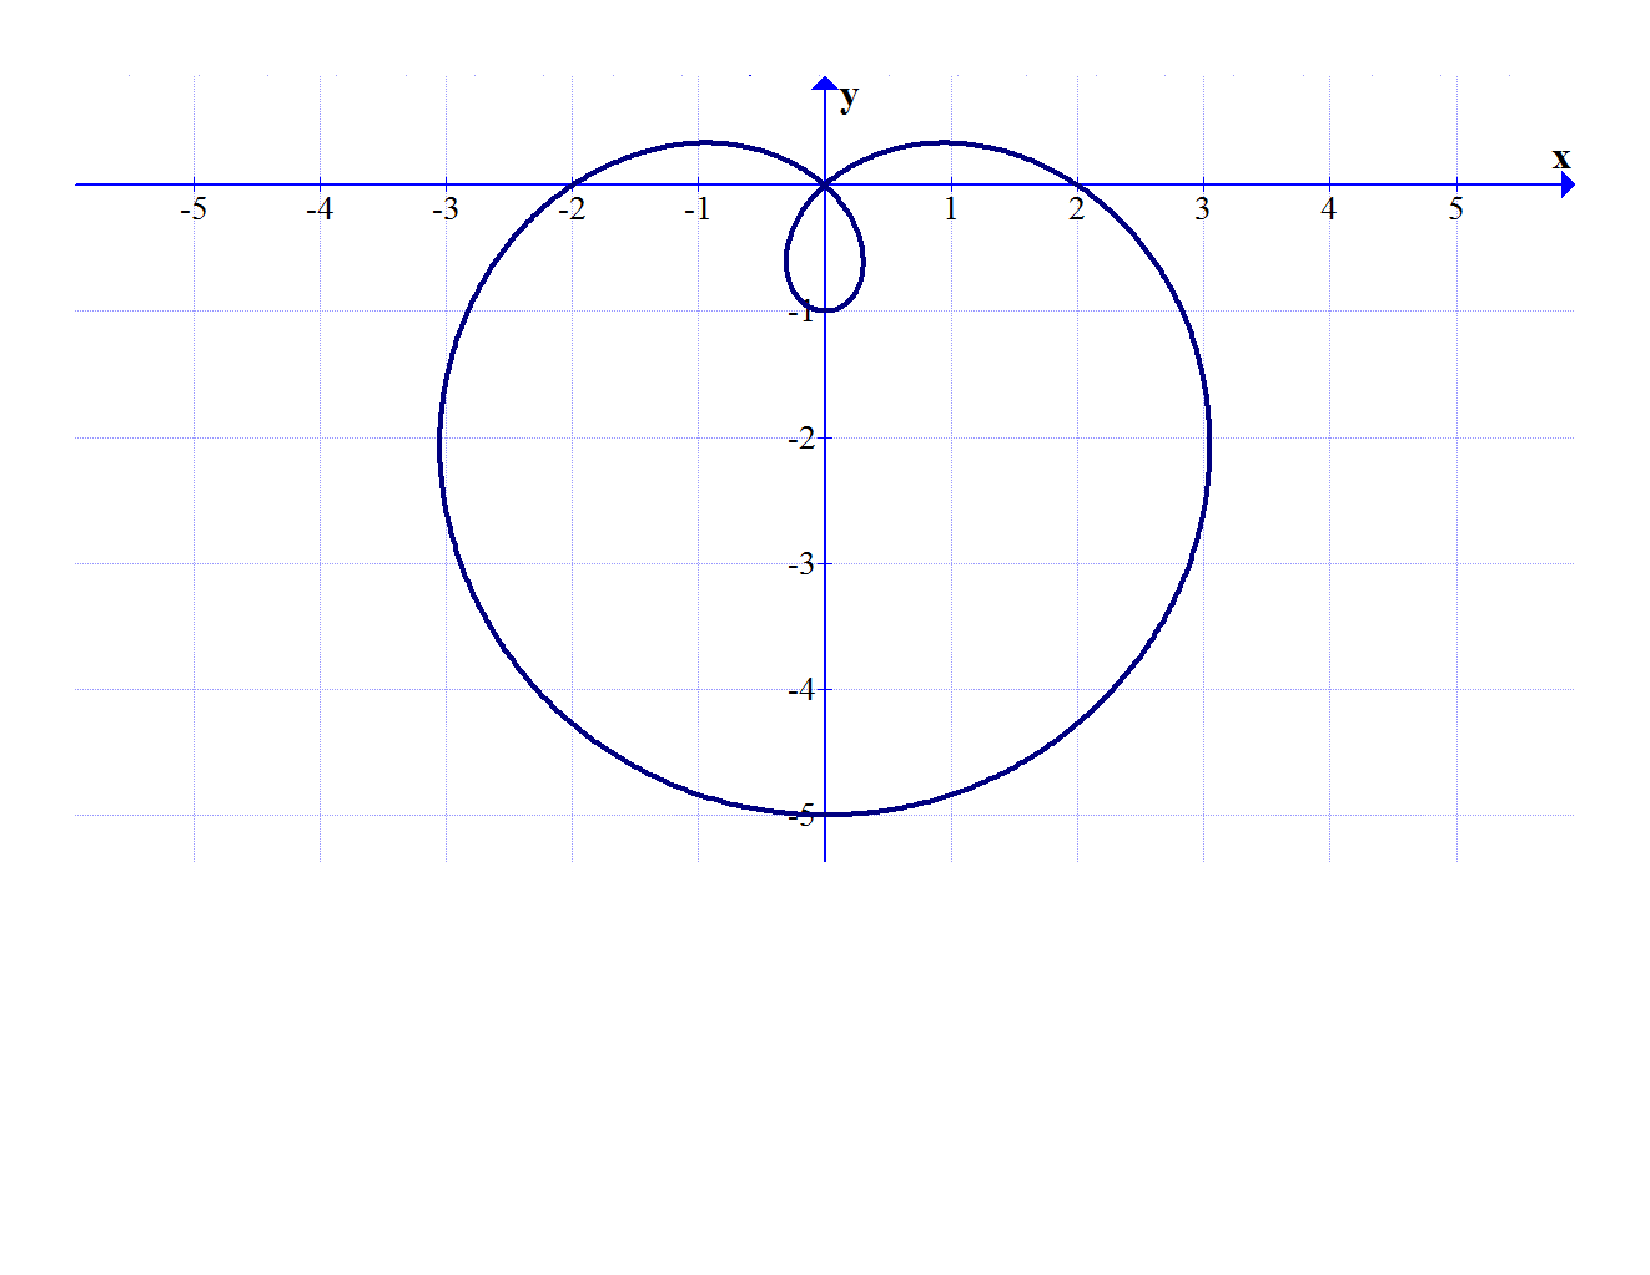
\includegraphics[scale=0.27]{sketch7.pdf}}} \fi

\item $r=2(1+\cos{\theta})$

\ifans{\fbox{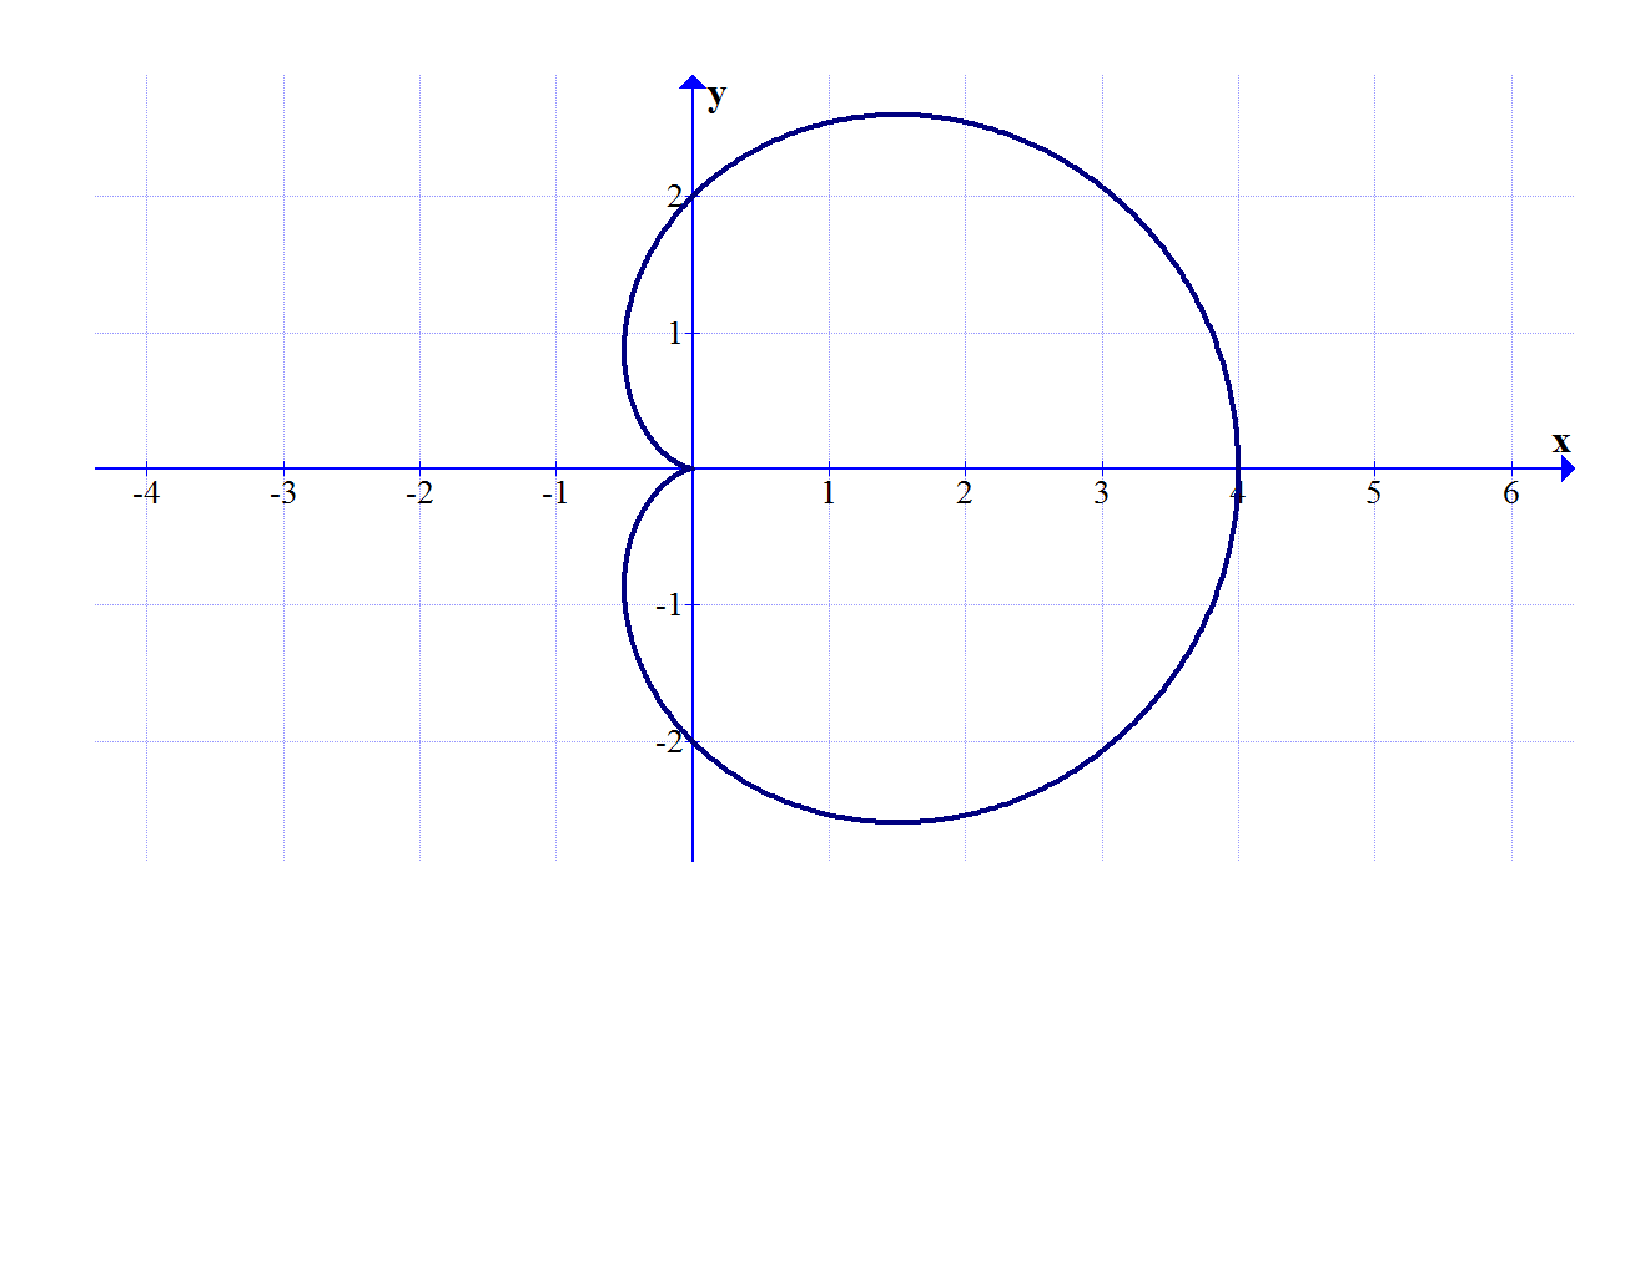
\includegraphics[scale=0.27]{sketch10.pdf}}} \fi

\newpage

\item $r=4\cos{2\theta}$ 

\ifans{\fbox{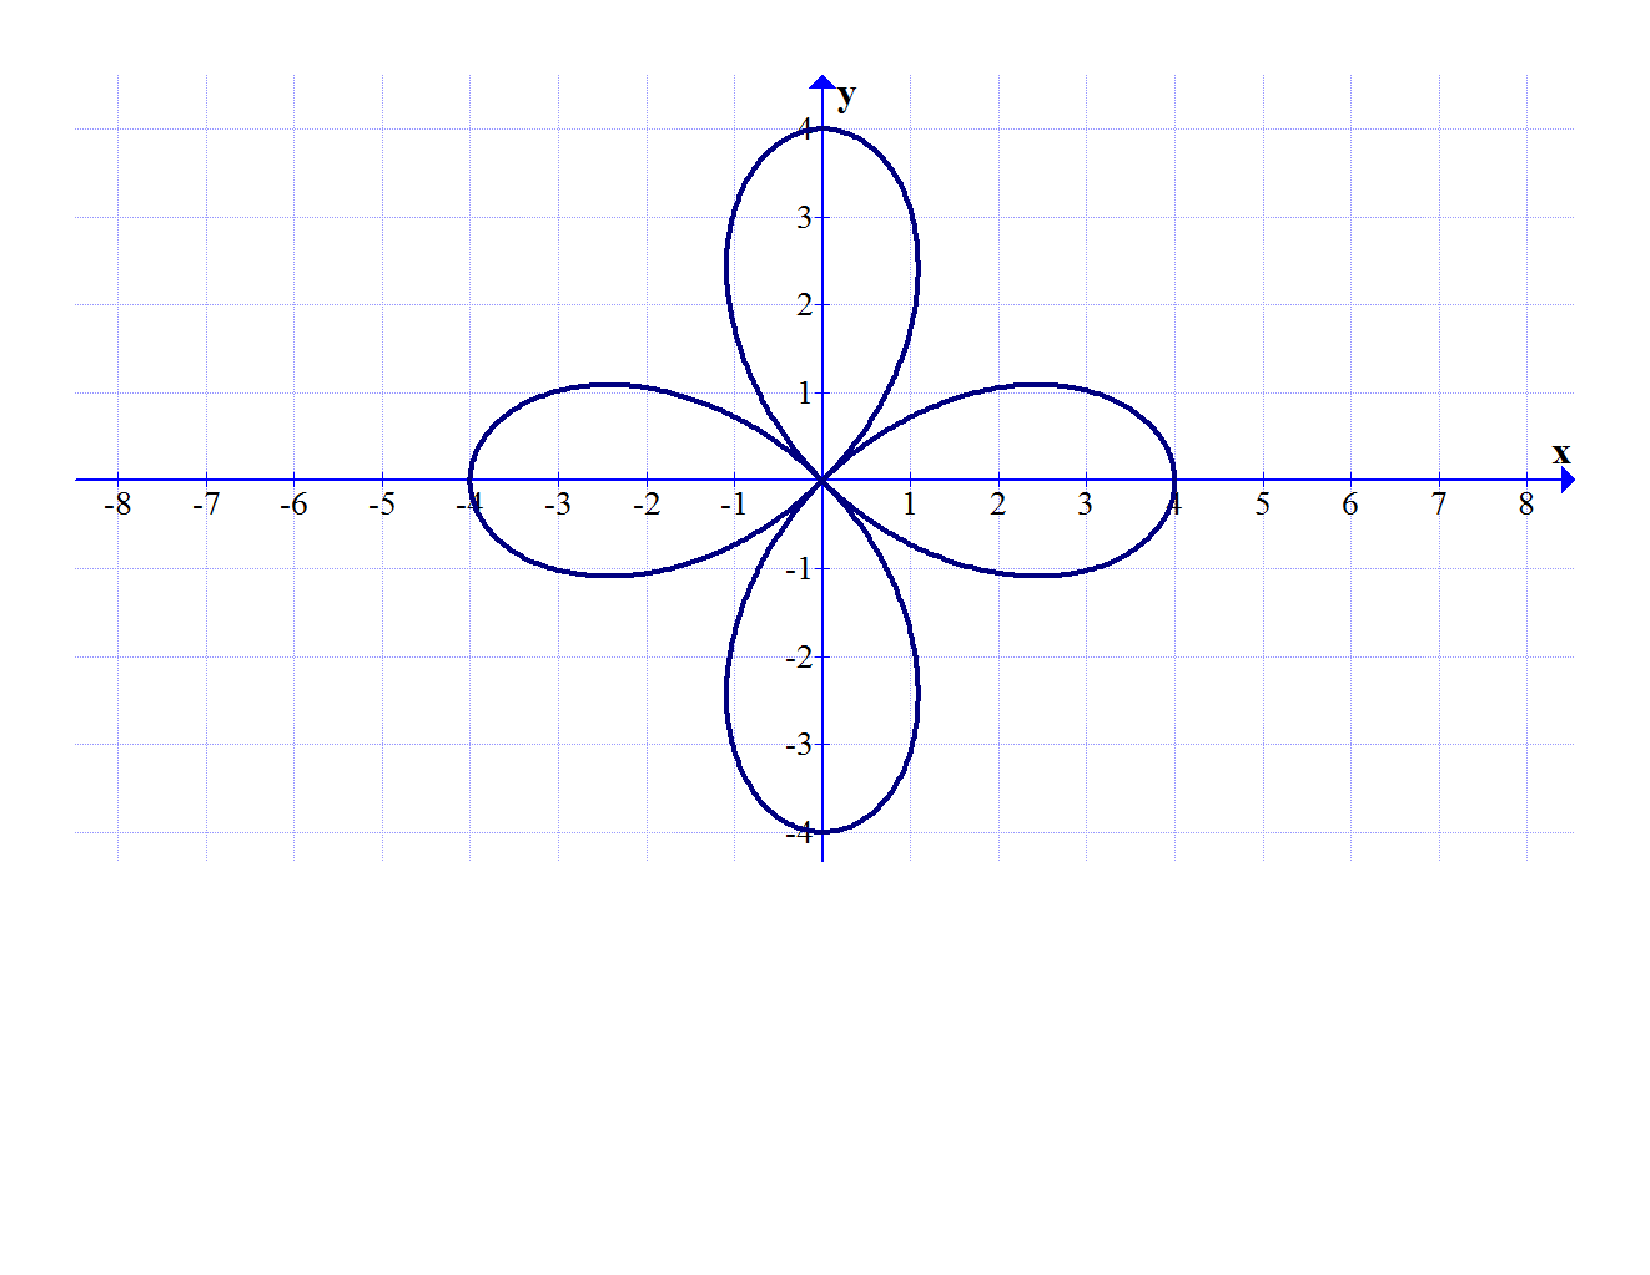
\includegraphics[scale=0.27]{sketch8.pdf}}} \fi

\item $r=-3\sin{3\theta}$ 

\ifans{\fbox{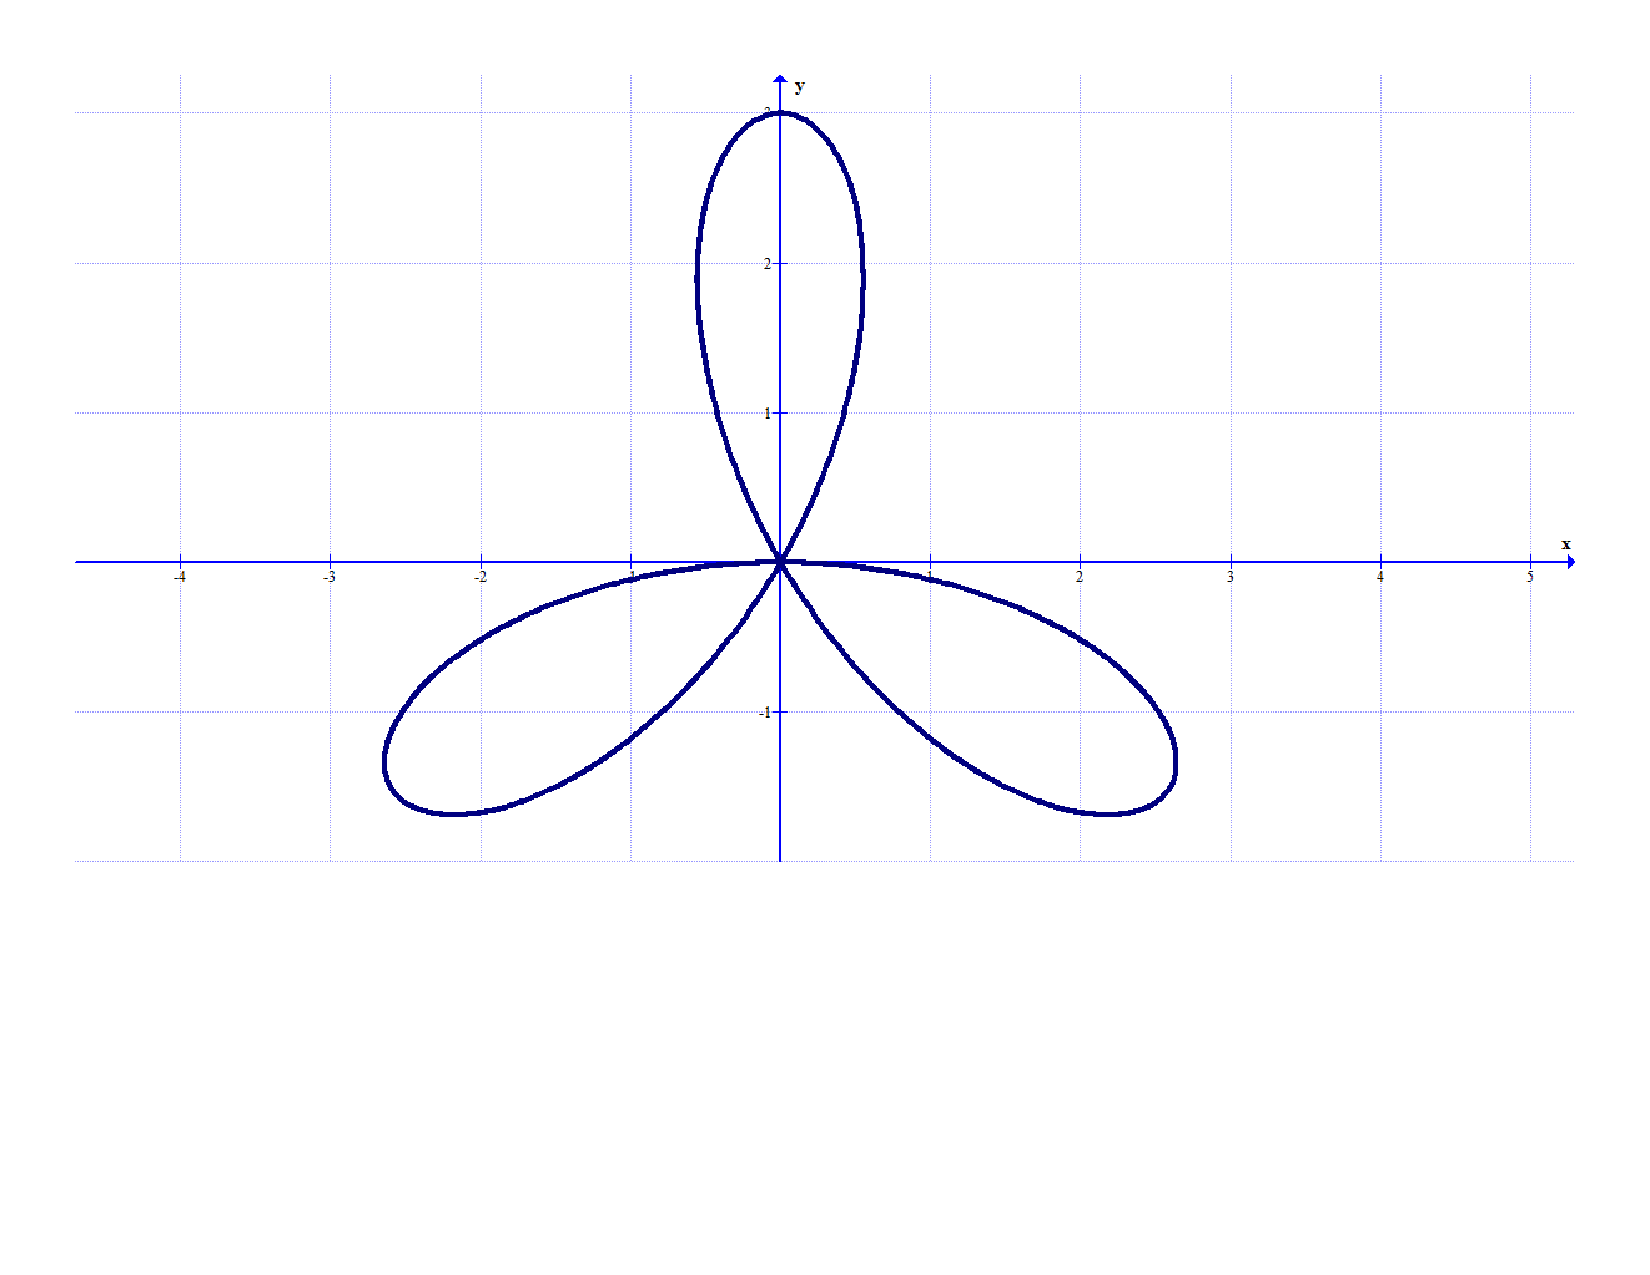
\includegraphics[scale=0.27]{sketch9.pdf}}} \fi

\end{enumerate}

\end{document}